\section{Background}
\label{s:context}

\begin{figure*}
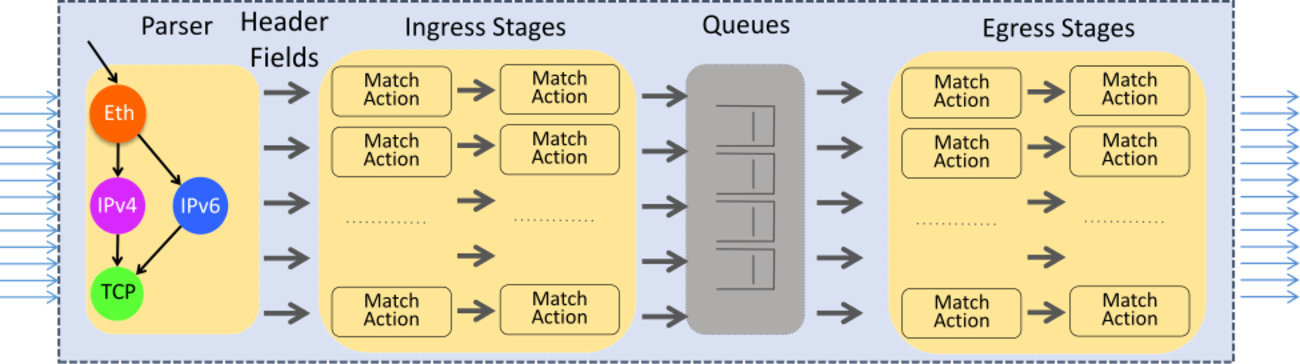
\includegraphics[width=\textwidth]{p4_switch_model.png}
\caption{The RMT architecture}
\end{figure*}

In this section we first review the architecture of
emerging programmable switches (\S\ref{ss:architecture}). We then describe the
class of data-plane algorithms that can be easily implemented using 
\pktlanguage's features (\S\ref{ss:dataplane}). 

%In the process, we observe that there is a large
%semantic gap between the high-level pseudocode style in which data-plane
%algorithms are available and low-level languages like P4 used to program
%pipelined switches today. This leads us to propose a high-level language and a
%compiler to bridge this gap.


\subsection{The architecture of a programmable switch}
\label{s:architecture}
In this section we briefly describe the Reconfigurable Match-Action Table (RMT)
architecture~\cite{rmt}, which is a representative programmable switch 
that is used in our experiments. Other switches with similar architecture include
Intel's FlexPipe~\cite{flexpipe} and Cavium's Xpliant~\cite{xpliant}.

Figure~\ref{fig:architecture} provides a
high-level overview of the RMT architecture. Packets enter the switch through
serial links and are handled by a programmable parser that turns packets into a
bag of header fields. The ingress and egress pipelines have a number of
physical pipeline stages that can process these header fields using a sequence
of match-action tables.
Such tables match on arbitrary header fields and carry out actions in response
to a match.  The actions are built out of simpler action primitives, which
represent simple arithmetic and logic operations on packet fields. To remain
performance competitive with fixed-function switches~\cite{mellanox, broadcom},
each action primitive can modify only one packet field, although several action
primitives can be grouped together into larger actions using a Very-Large
Instruction Word if they can all execute in parallel without violating data
dependencies such as XXX read-after-write.

The RMT architecture also includes a set of atomic stateful operations, i.e., 
operations that allow packets to manipulate persistent state atomically from
one packet to the next.  We summarize these in
Table~\ref{t:stateful_inst}.\footnote{We use the symbols {\tt x} %and {\tt y} 
\ac{table doesn't use y} to refer to
stateful variables and {\tt pkt.<>} to refer to a packet field.
{\tt pkt.field} can be substituted for a constant operand in places that are appropriate.}
\begin{table}
\begin{small}
\begin{tabular}{|c|c|}
\hline
Instruction description & Form \\
\hline
Read and write & \texttt{x = pkt.field;} or \texttt{pkt.field = x;} \\
\hline
Read, modify, and write & \texttt{x = x + pkt.field;} \\
\hline
Conditional execution & \texttt{x = pkt.predicate ? pkt.field : x;} \\
\hline
\end{tabular}
\end{small}
\caption{Atmoic stateful instructions in the RMT architecture}
\label{t:stateful_inst}
\end{table}
%\item Packed operations on pairs of stateful variables: \texttt{ (x, y) = (x + y, x - y);}
%\item Multiply and accumulate a stateful variable: \texttt{ x = x * pkt.field + pkt.field2; }

RMT is a shared-nothing architecture: state variables are local to a particular
stage in the ingress or egress pipeline and cannot be shared across pipeline
stages or pipelines. 
% Alvin: I think these are too low level details that are unnecessary
%If a state variable were to be accessed from multiple
%stages, the underlying memory would need to support more than 1
%Read-Modify-Write per clock cycle. Embedded on-chip memory banks typically
%support only 1 Read-Modify-Write operation per clock
%cycle~\cite{some_citation_from_memoir} because building multi-ported RAMs is
%power and area hungry.
Instead, the RMT architecture allows communication between stages by cloning a
packet and recirculating it back into a pipeline \ac{I thought this is only needed
to communicate between a stage and its predecessors. For successor stages isn't
packet temporaries sufficient?}.
Now, a state variable can
be read in stage x, written downstream in stage y, and then a cloned packet to
stage x could update the state variable in x. However, this has a cost:
recirculated packets consume pipeline capacity by taking away capacity from
new data packets. Further, recirculation latency can be large: several hundred
packets might pass through the pipeline before the recirculated packet update
state in stage x.

\subsection{Data-plane Algorithms}
\label{ss:data-plane}
 We focus on data-plane algorithms that aren't widely available on all switches
today because of the considerable engineering effort required for hardware
implementations and the rapidly changing nature of these algorithms. For
instance, load-balancing algorithms such as CONGA~\cite{conga} are available
only on a specific line of CISCO switches.  Active queue-management algorithms
such as CoDel~\cite{codel} need to be extensively modified~\cite{pie} to suit
the architecture of a hardware switch.  Explicit congestion-control algorithms
such as RCP~\cite{rcp} and XCP~\cite{xcp}, and measurement algorithms such as
OpenSketch~\cite{opensketch} have been evaluated only in FPGA-based platforms.
The ever-growing list of new algorithms~\cite{pdq, d3, detail} makes it
challenging to commit to a hardware implementation of any of them.

 Programmable switches present us with an alternative: we could
\textit{program} a switch pipeline to express a new algorithm as opposed to
implementing it anew in hardware.

One approach to program these data-plane algorithms is to use a
packet-processing language such as P4, which compiles to several targets such
as the RMT architecture and Intel's FlexPipe
architecture~\cite{lavanya_compiler}. However, P4 in its current form, matches
the structure of its hardware targets: the action primitives in P4 correspond
1:1 to action primitives available in the hardware and its abstract switch
model is very similar to a switch pipeline.

While these decisions ease the job of the P4 compiler, they make it harder for
a programmer to write code in P4---something that we have struggled with for
several of the algorithms presented above. A closer inspection of these
algorithms shows us that the algorithms are characterized by two distinguishing
features: a reliance on persistant state and an irregular control flow, both of
which make them challenging to implement in hardware and hence in P4 given its
low-level nature.

However, given the growing adoption of P4, we think it prudent to leverage
existing work on P4 compilation to hardware targets~\cite{netronome, xilinx}.
With this in mind, our work focuses on building a compiler from \pktlanguage to
P4, letting P4 address the backend problem of table placement that is unique to
each target architecture~\cite{lavanya_compiler}.
